\documentclass[tikz,border=4pt]{standalone}
\usepackage{amsmath}
\begin{document}
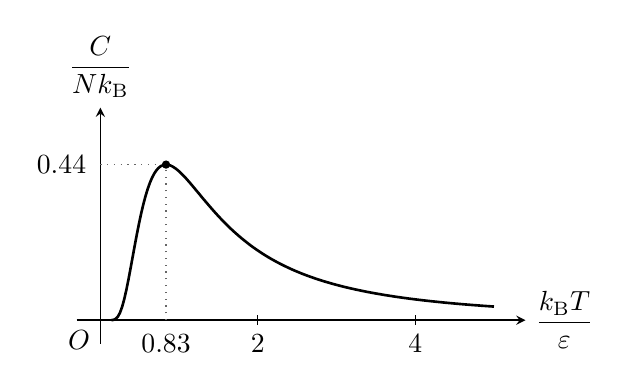
\begin{tikzpicture}[>=stealth, thick, scale=1.0]
  % Axes: x = k_B T / eps (0 to 5), y = C / (N k_B) (scaled by 4.5 so peak 0.439 -> 1.98)
  \draw[->, line width=0.5pt] (-0.3, 0) -- (5.4, 0) node[right] {$\dfrac{k_{\mathrm{B}}T}{\varepsilon}$};
  \draw[->, line width=0.5pt] (0, -0.3) -- (0, 2.7) node[above] {$\dfrac{C}{Nk_{\mathrm{B}}}$};
  \node[below left] at (0, 0) {$O$};

  % Plot y = 4.5 * (1/x)^2 / cosh^2(1/x) for x in [0.14, 5.0]
  \draw[line width=0.95pt] (0, 0) -- (0.14, 0);
  \draw[line width=0.95pt, domain=0.14:5.0, samples=180]
    plot (\x, {4.5 * ((1/\x) / cosh(1/\x))^2});

  % Peak at x = 0.834, y_val = 0.439 -> plot y = 1.976
  \draw[dotted, line width=0.45pt, black!60] (0.834, 0) -- (0.834, 1.976);
  \draw[dotted, line width=0.45pt, black!60] (0, 1.976) -- (0.834, 1.976);
  \fill (0.834, 1.976) circle (1.5pt);
  \node[below] at (0.834, -0.05) {$0.83$};
  \node[left] at (-0.05, 1.976) {$0.44$};

  % Ticks on x-axis
  \foreach \xt in {2, 4} {
    \draw[line width=0.4pt] (\xt, 0.06) -- (\xt, -0.06) node[below] {$\xt$};
  }
\end{tikzpicture}
\end{document}
